%!TEX root = ../../master.tex

\subsection*{Visualizer}
Visualization is expected to play an important role in students' learning and the bridging between cloud computing and the physical machines, especially since engineering students tend to be visual learners. This fulfils the requirement \textit{"KubeCloud shall be able to visualize the state of the cluster"}. KubeCloud allows for injecting failures e.g. by pulling the network cables (Figure~\ref{fig:visualizer_node_failure}). However, it can be hard to understand and grasp what is going on in Kubernetes. Hence, a visualization tool is needed. 

\begin{figure}[H]%
    \centering
    \subfloat[Node failure]{{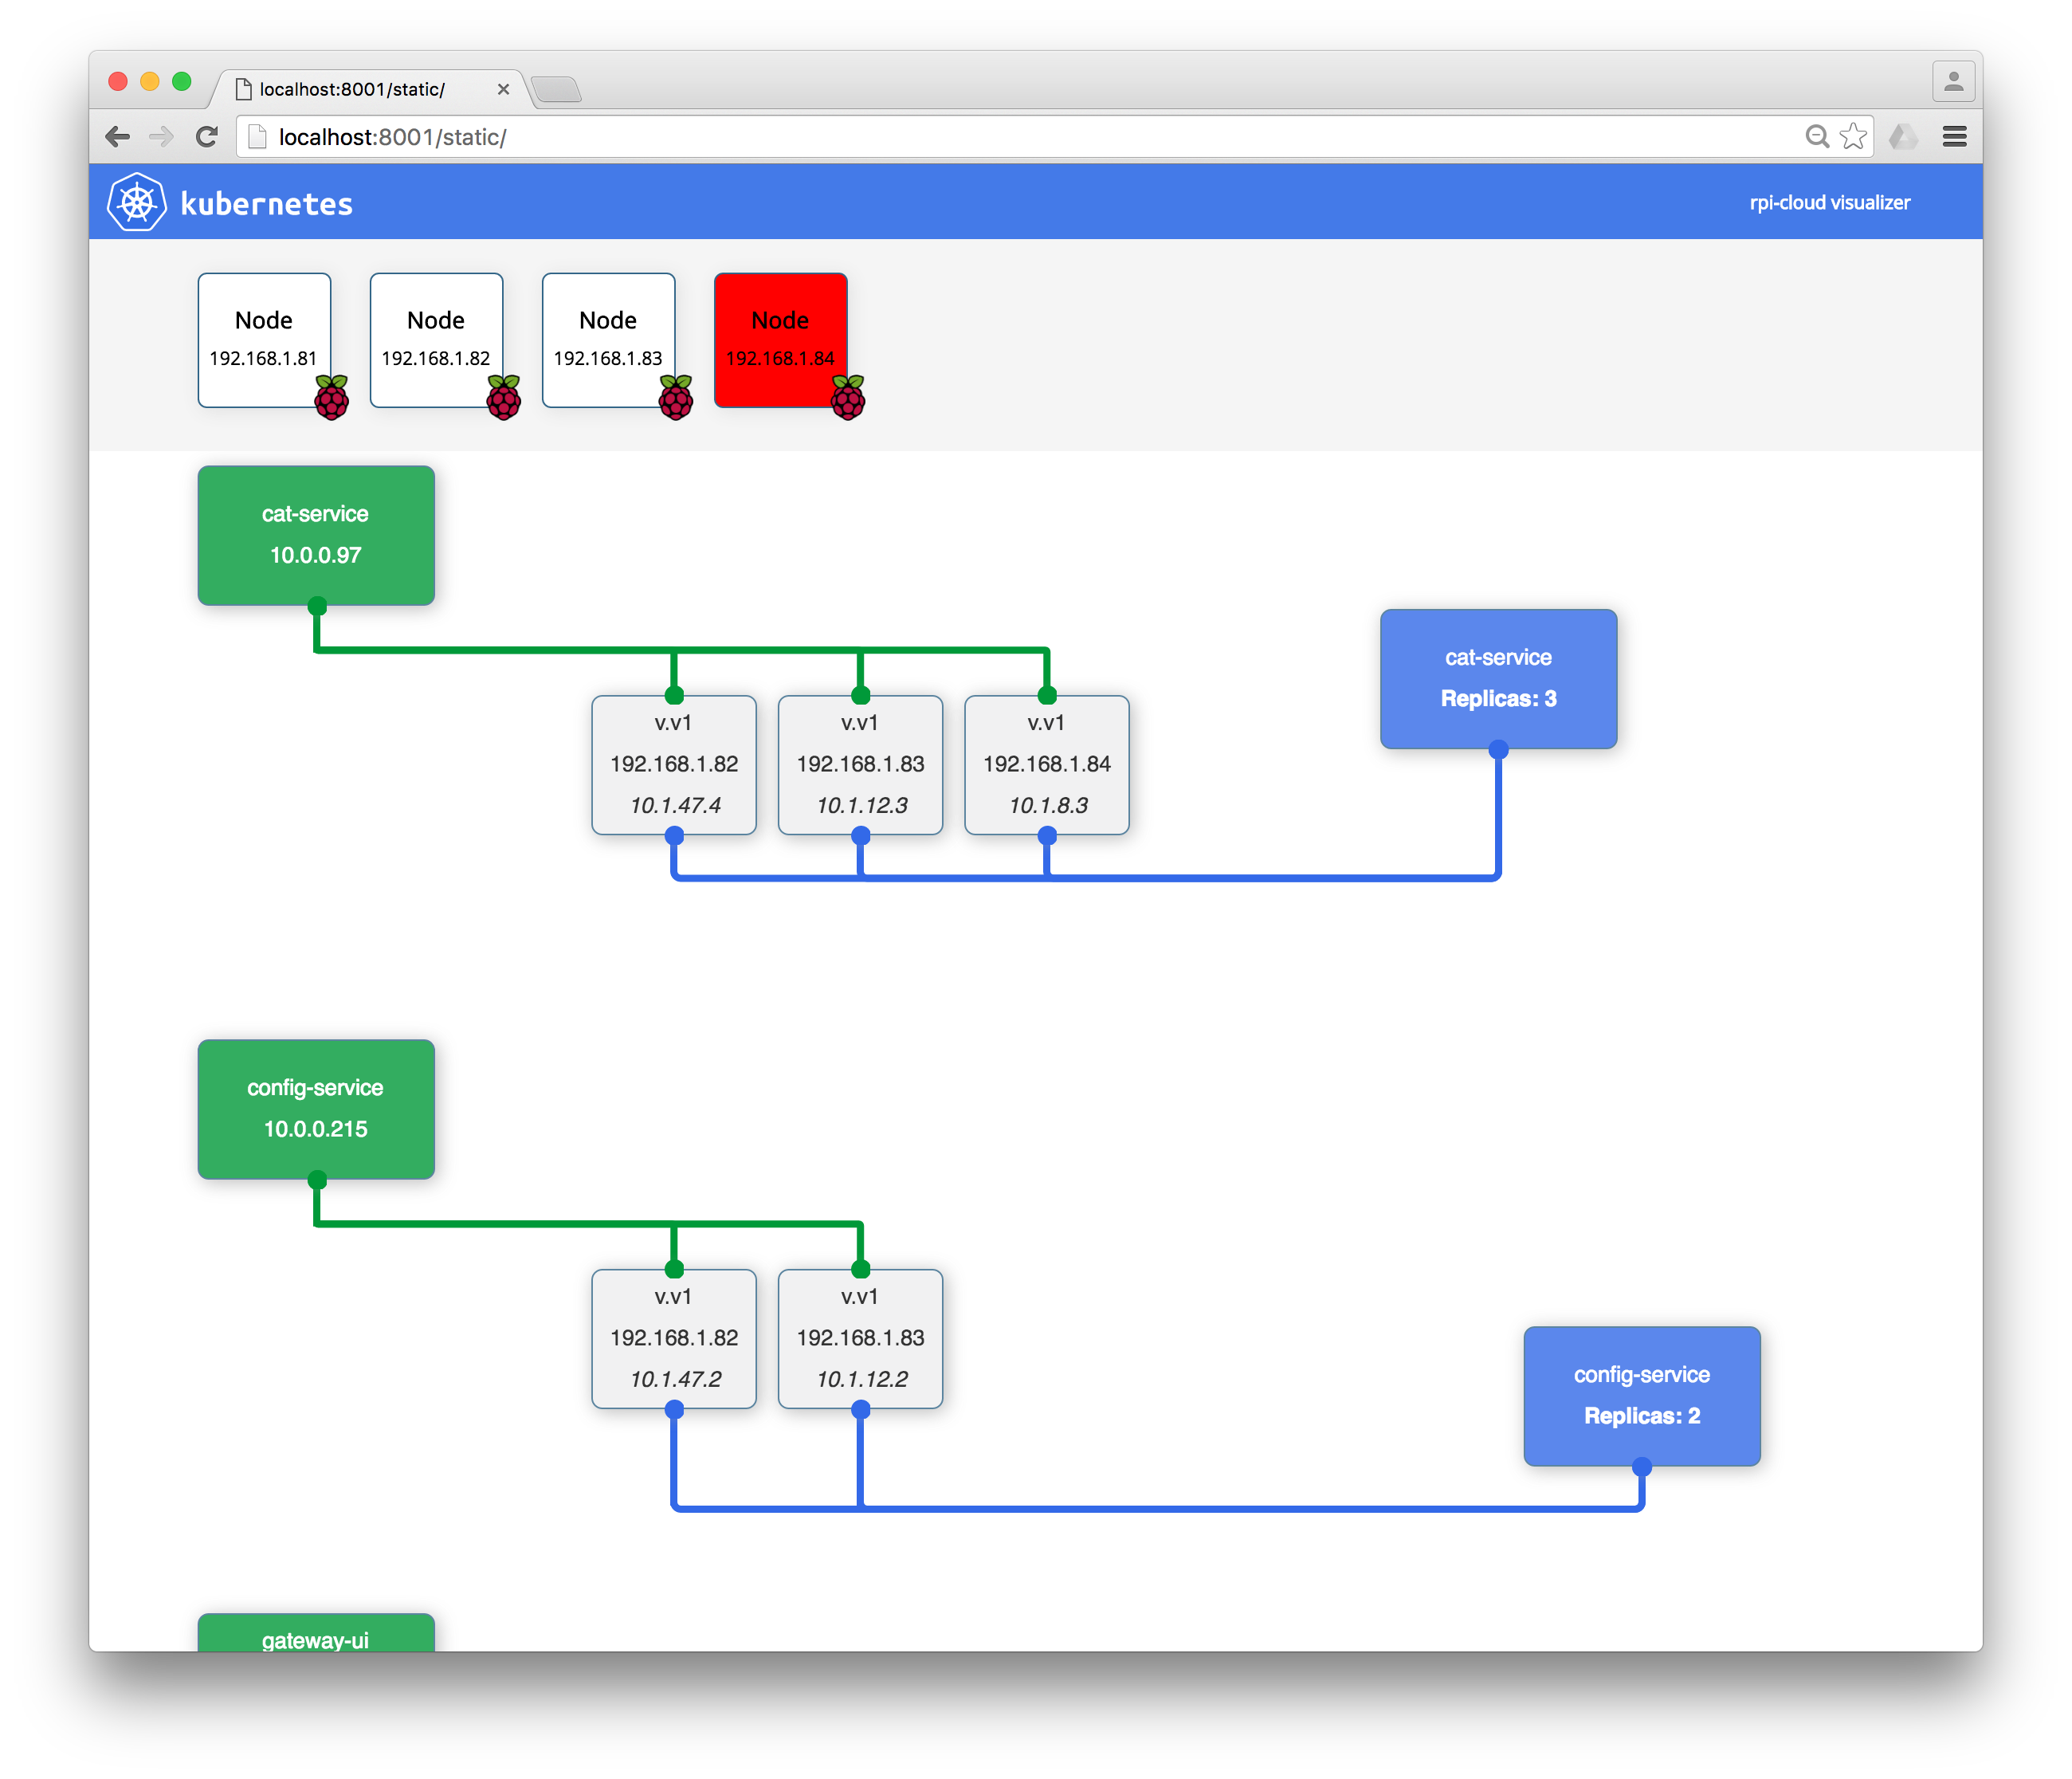
\includegraphics[width=7cm]{figures/visualizer/node_fail} }}%
      \qquad
    \subfloat[Rescheduling]{{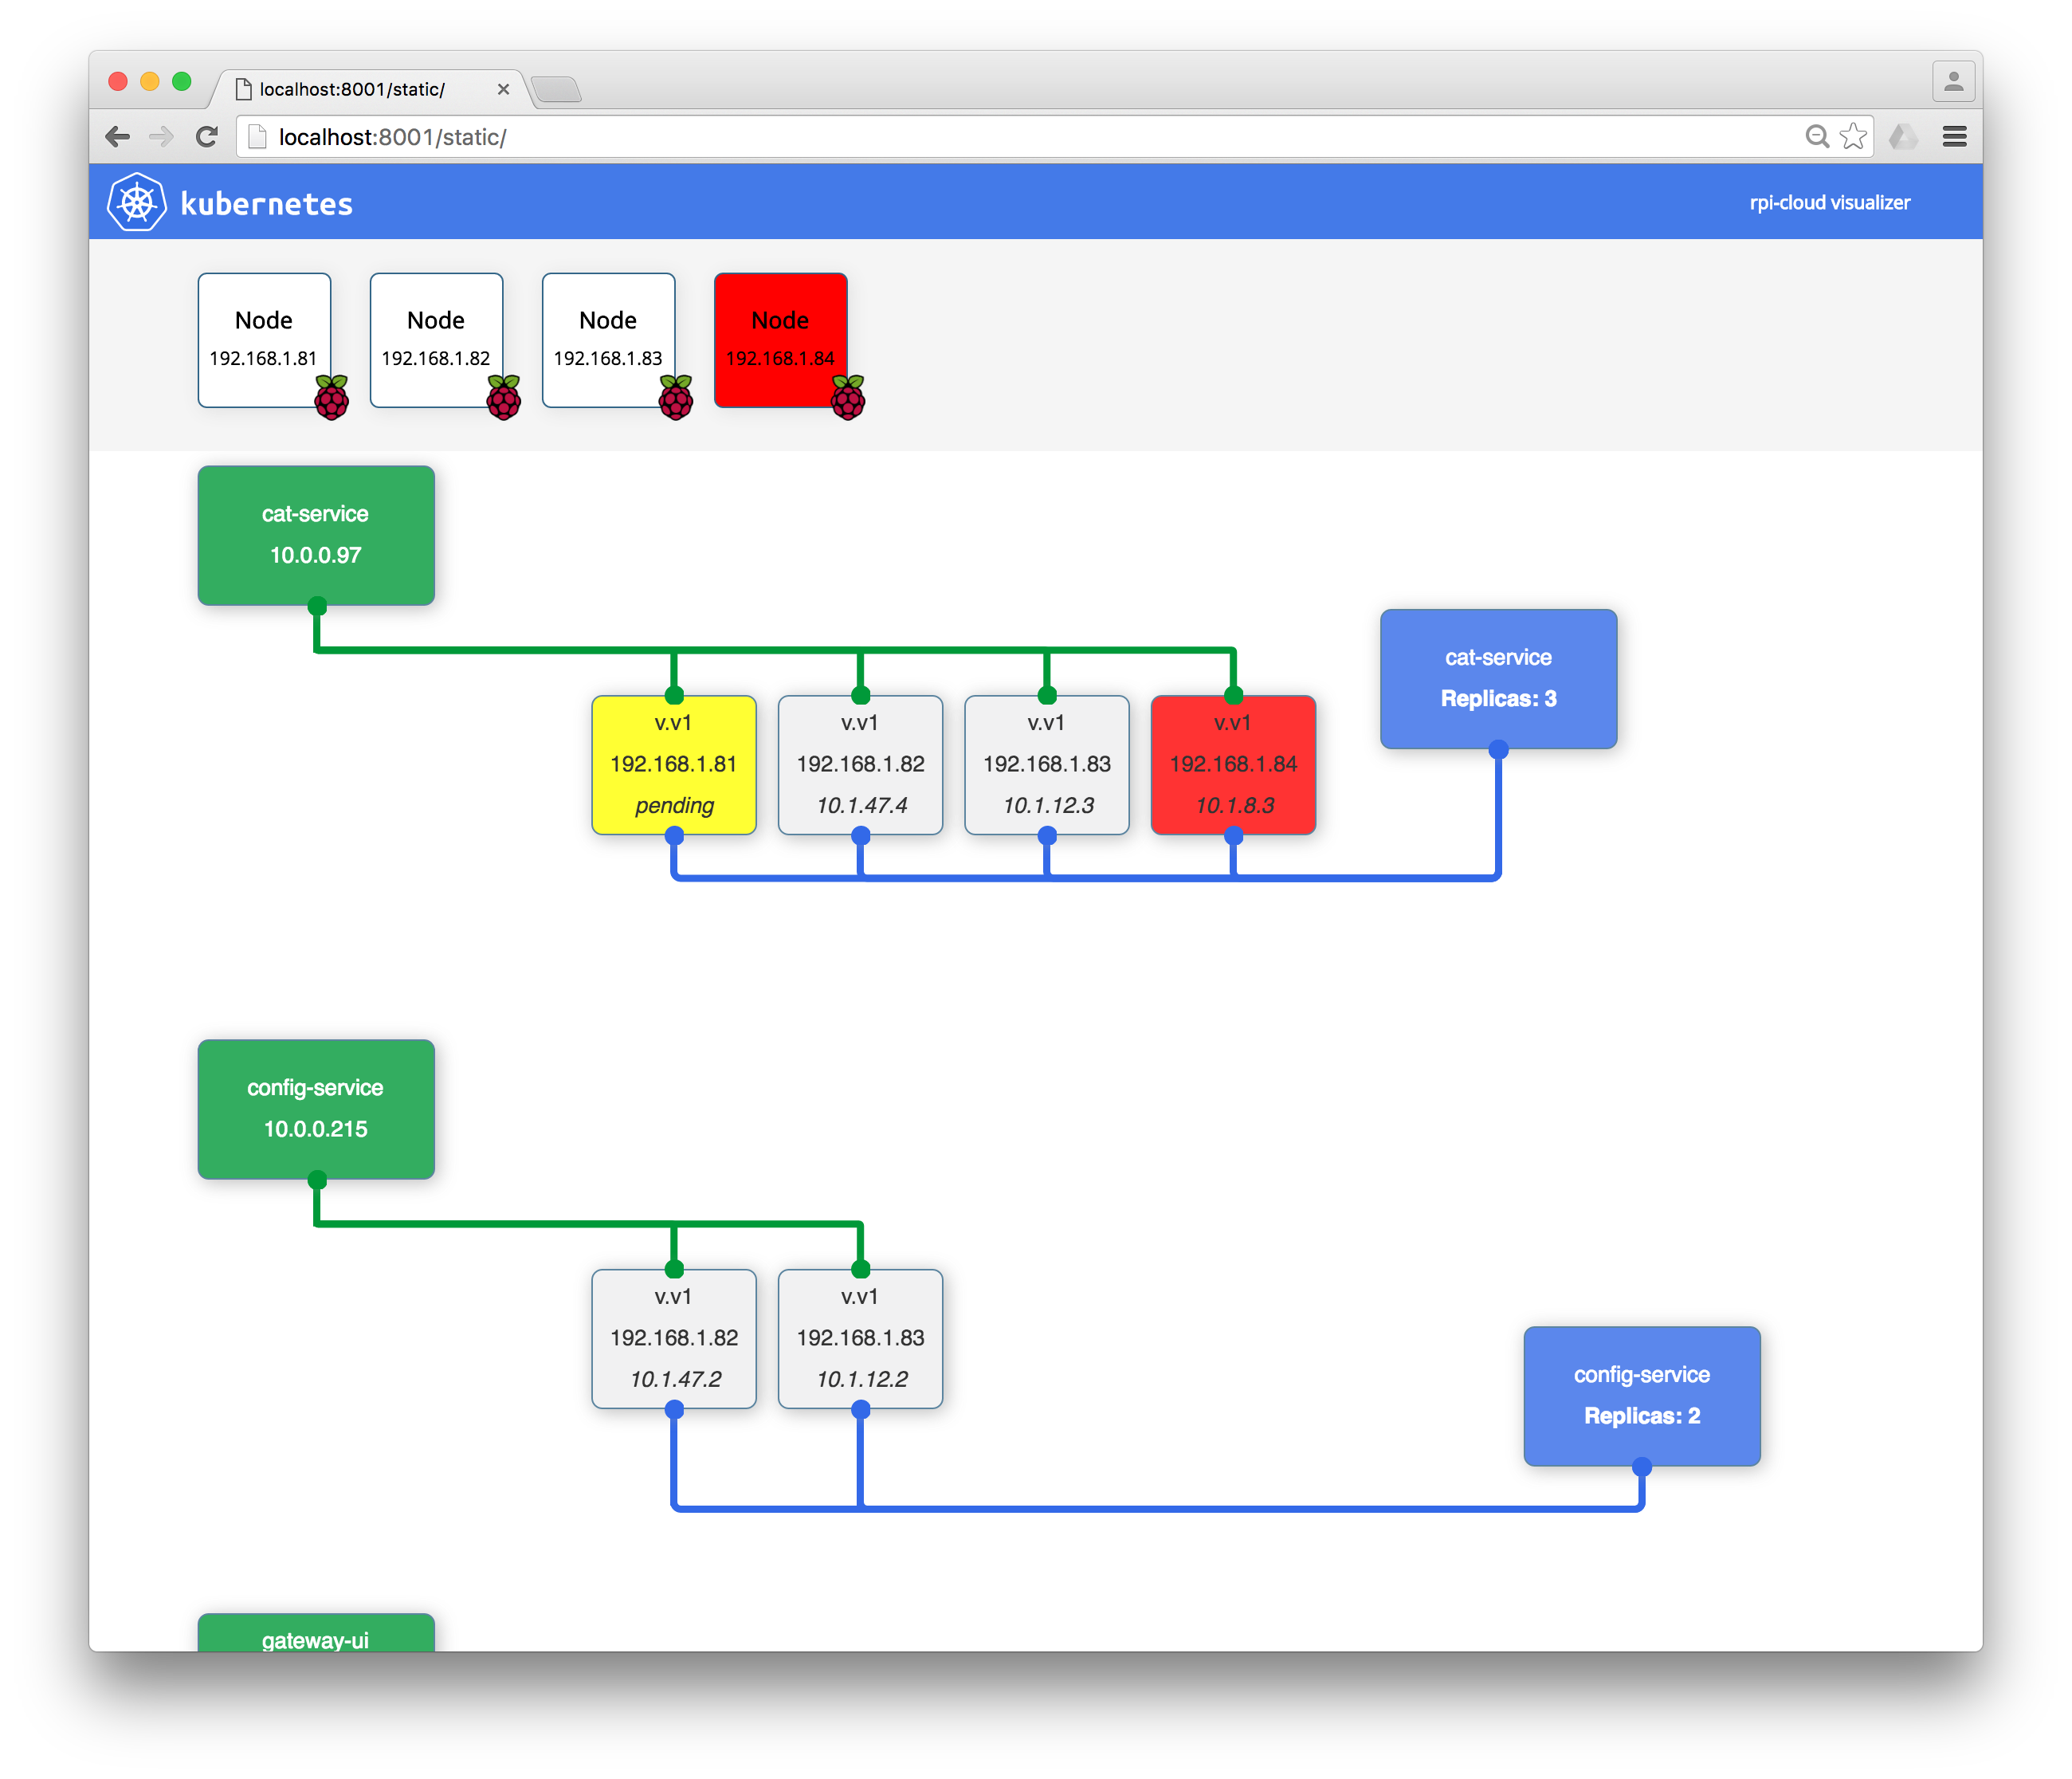
\includegraphics[width=7cm]{figures/visualizer/node_fail_reschedule} }}%
          \qquad
    \subfloat[Recovered]{{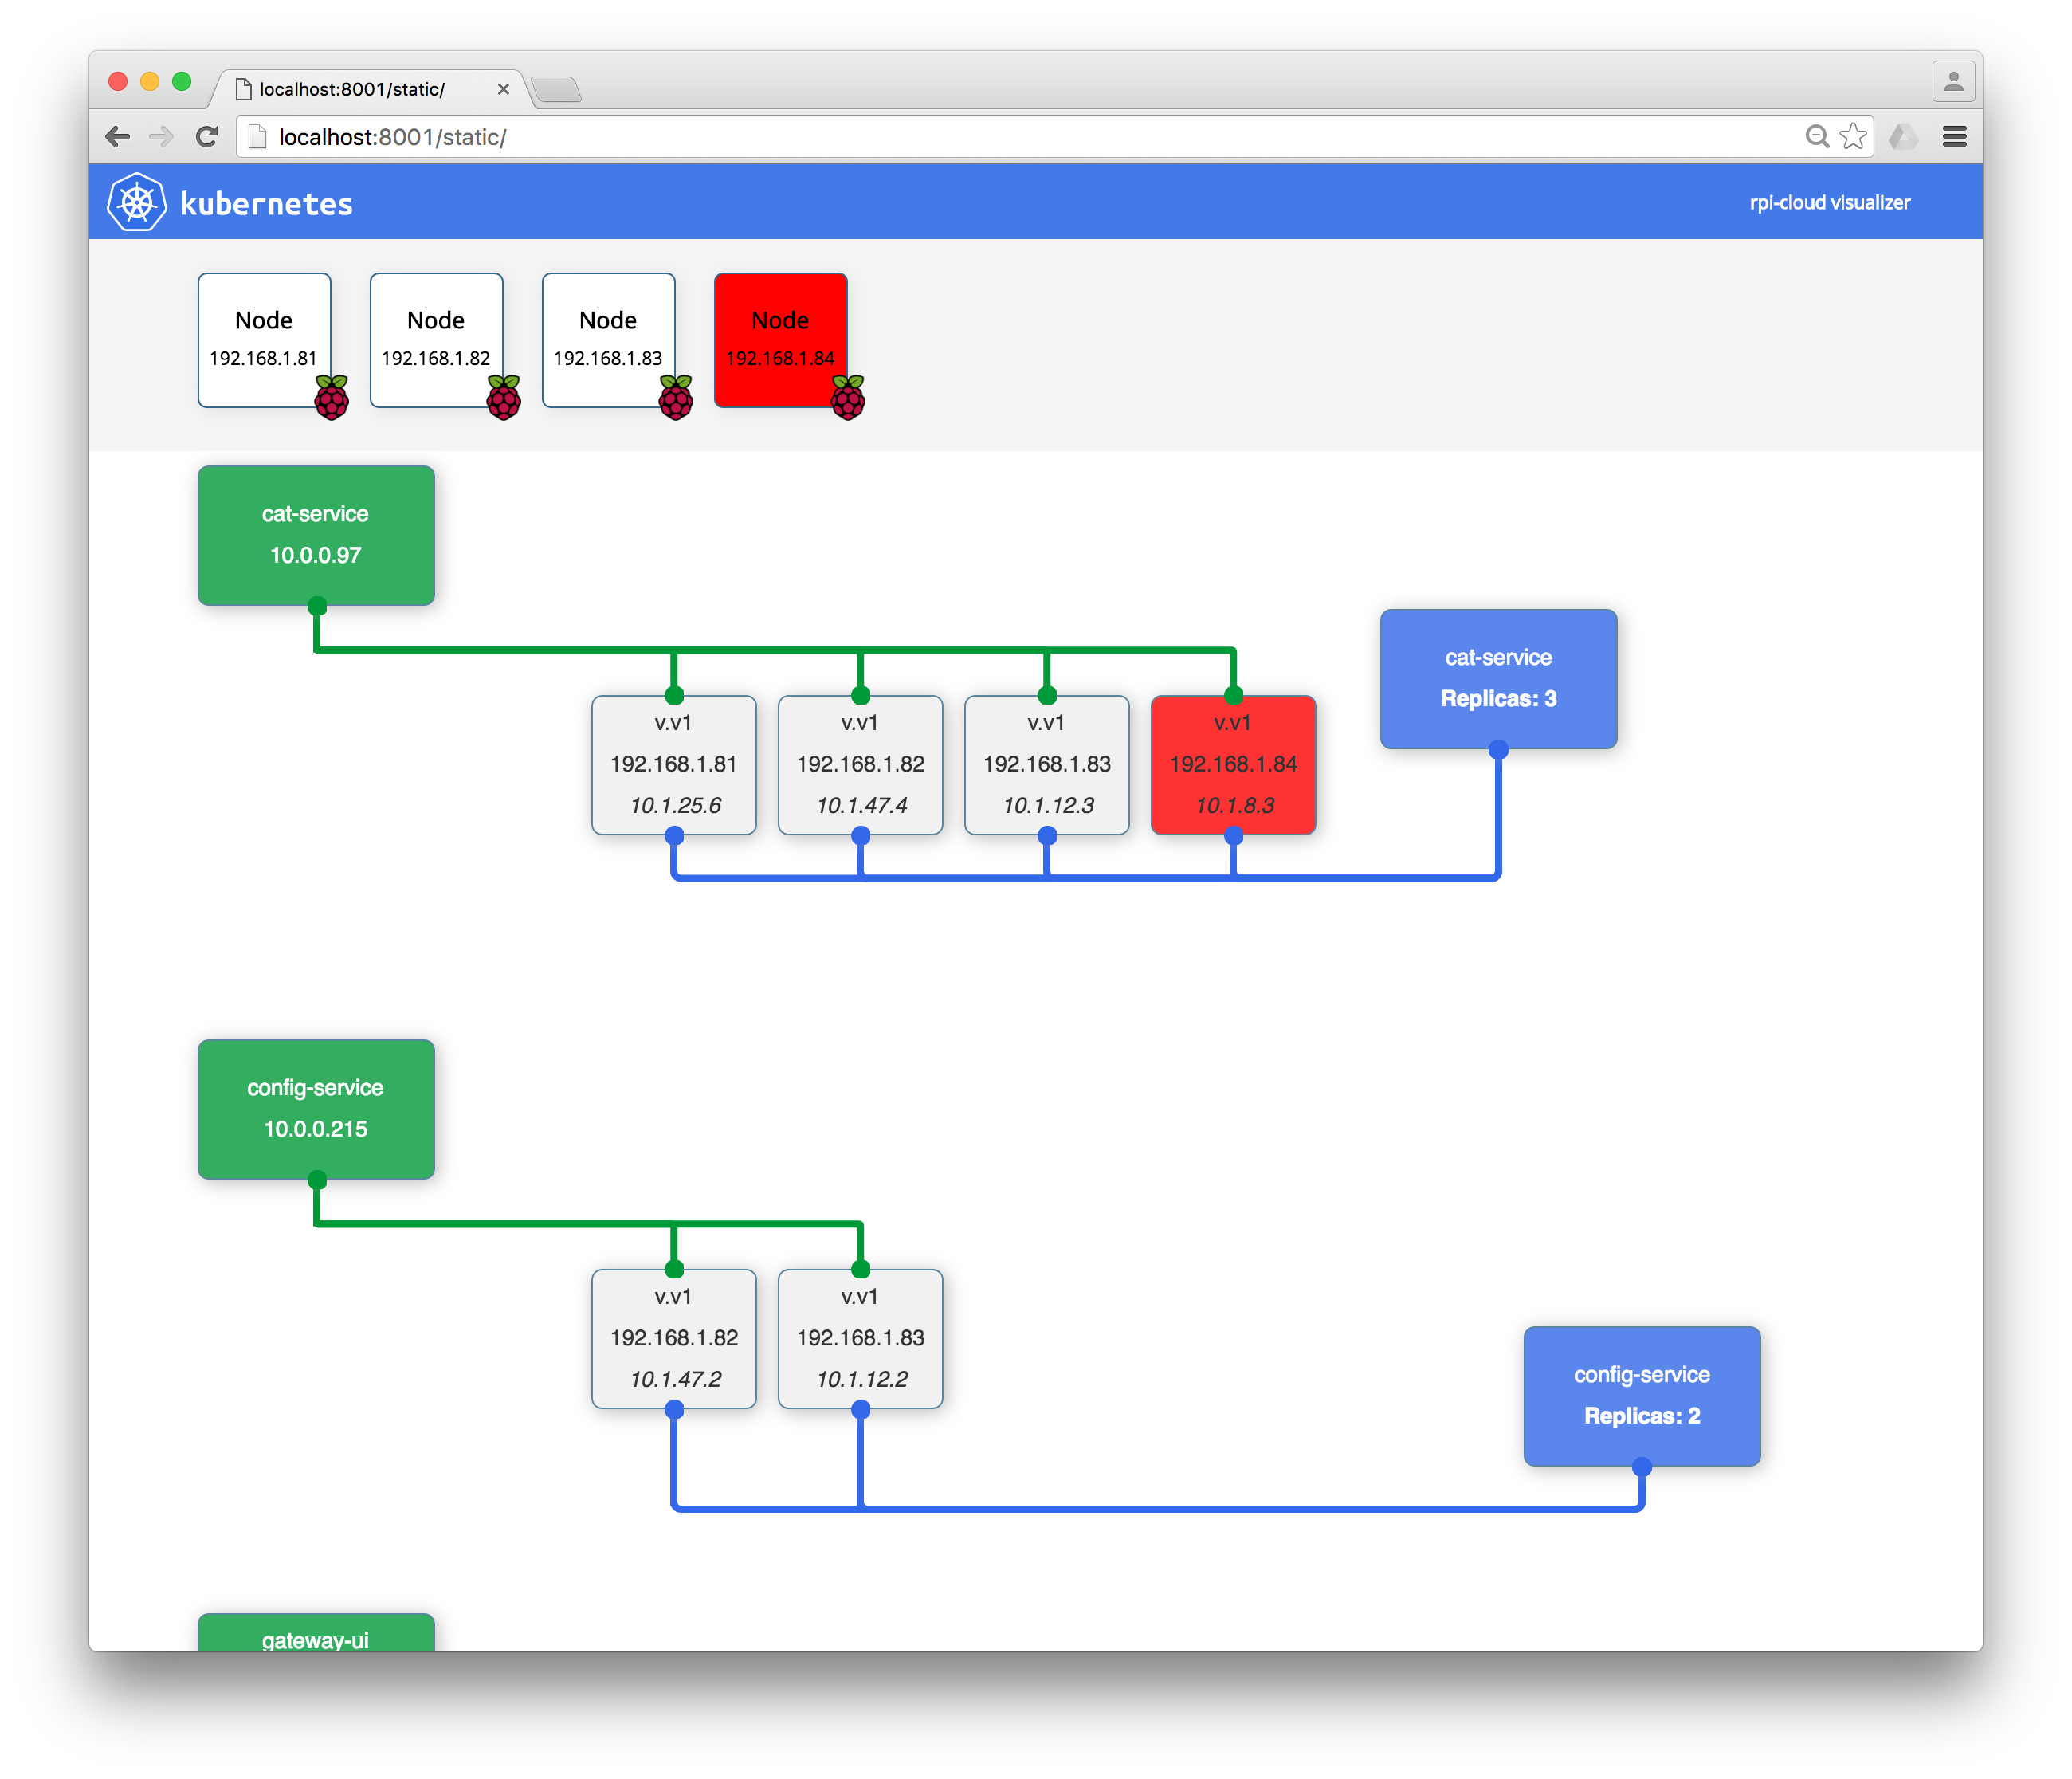
\includegraphics[width=7cm]{figures/visualizer/node_fail_clean_up} }}%
          \qquad
    \subfloat[Clean up]{{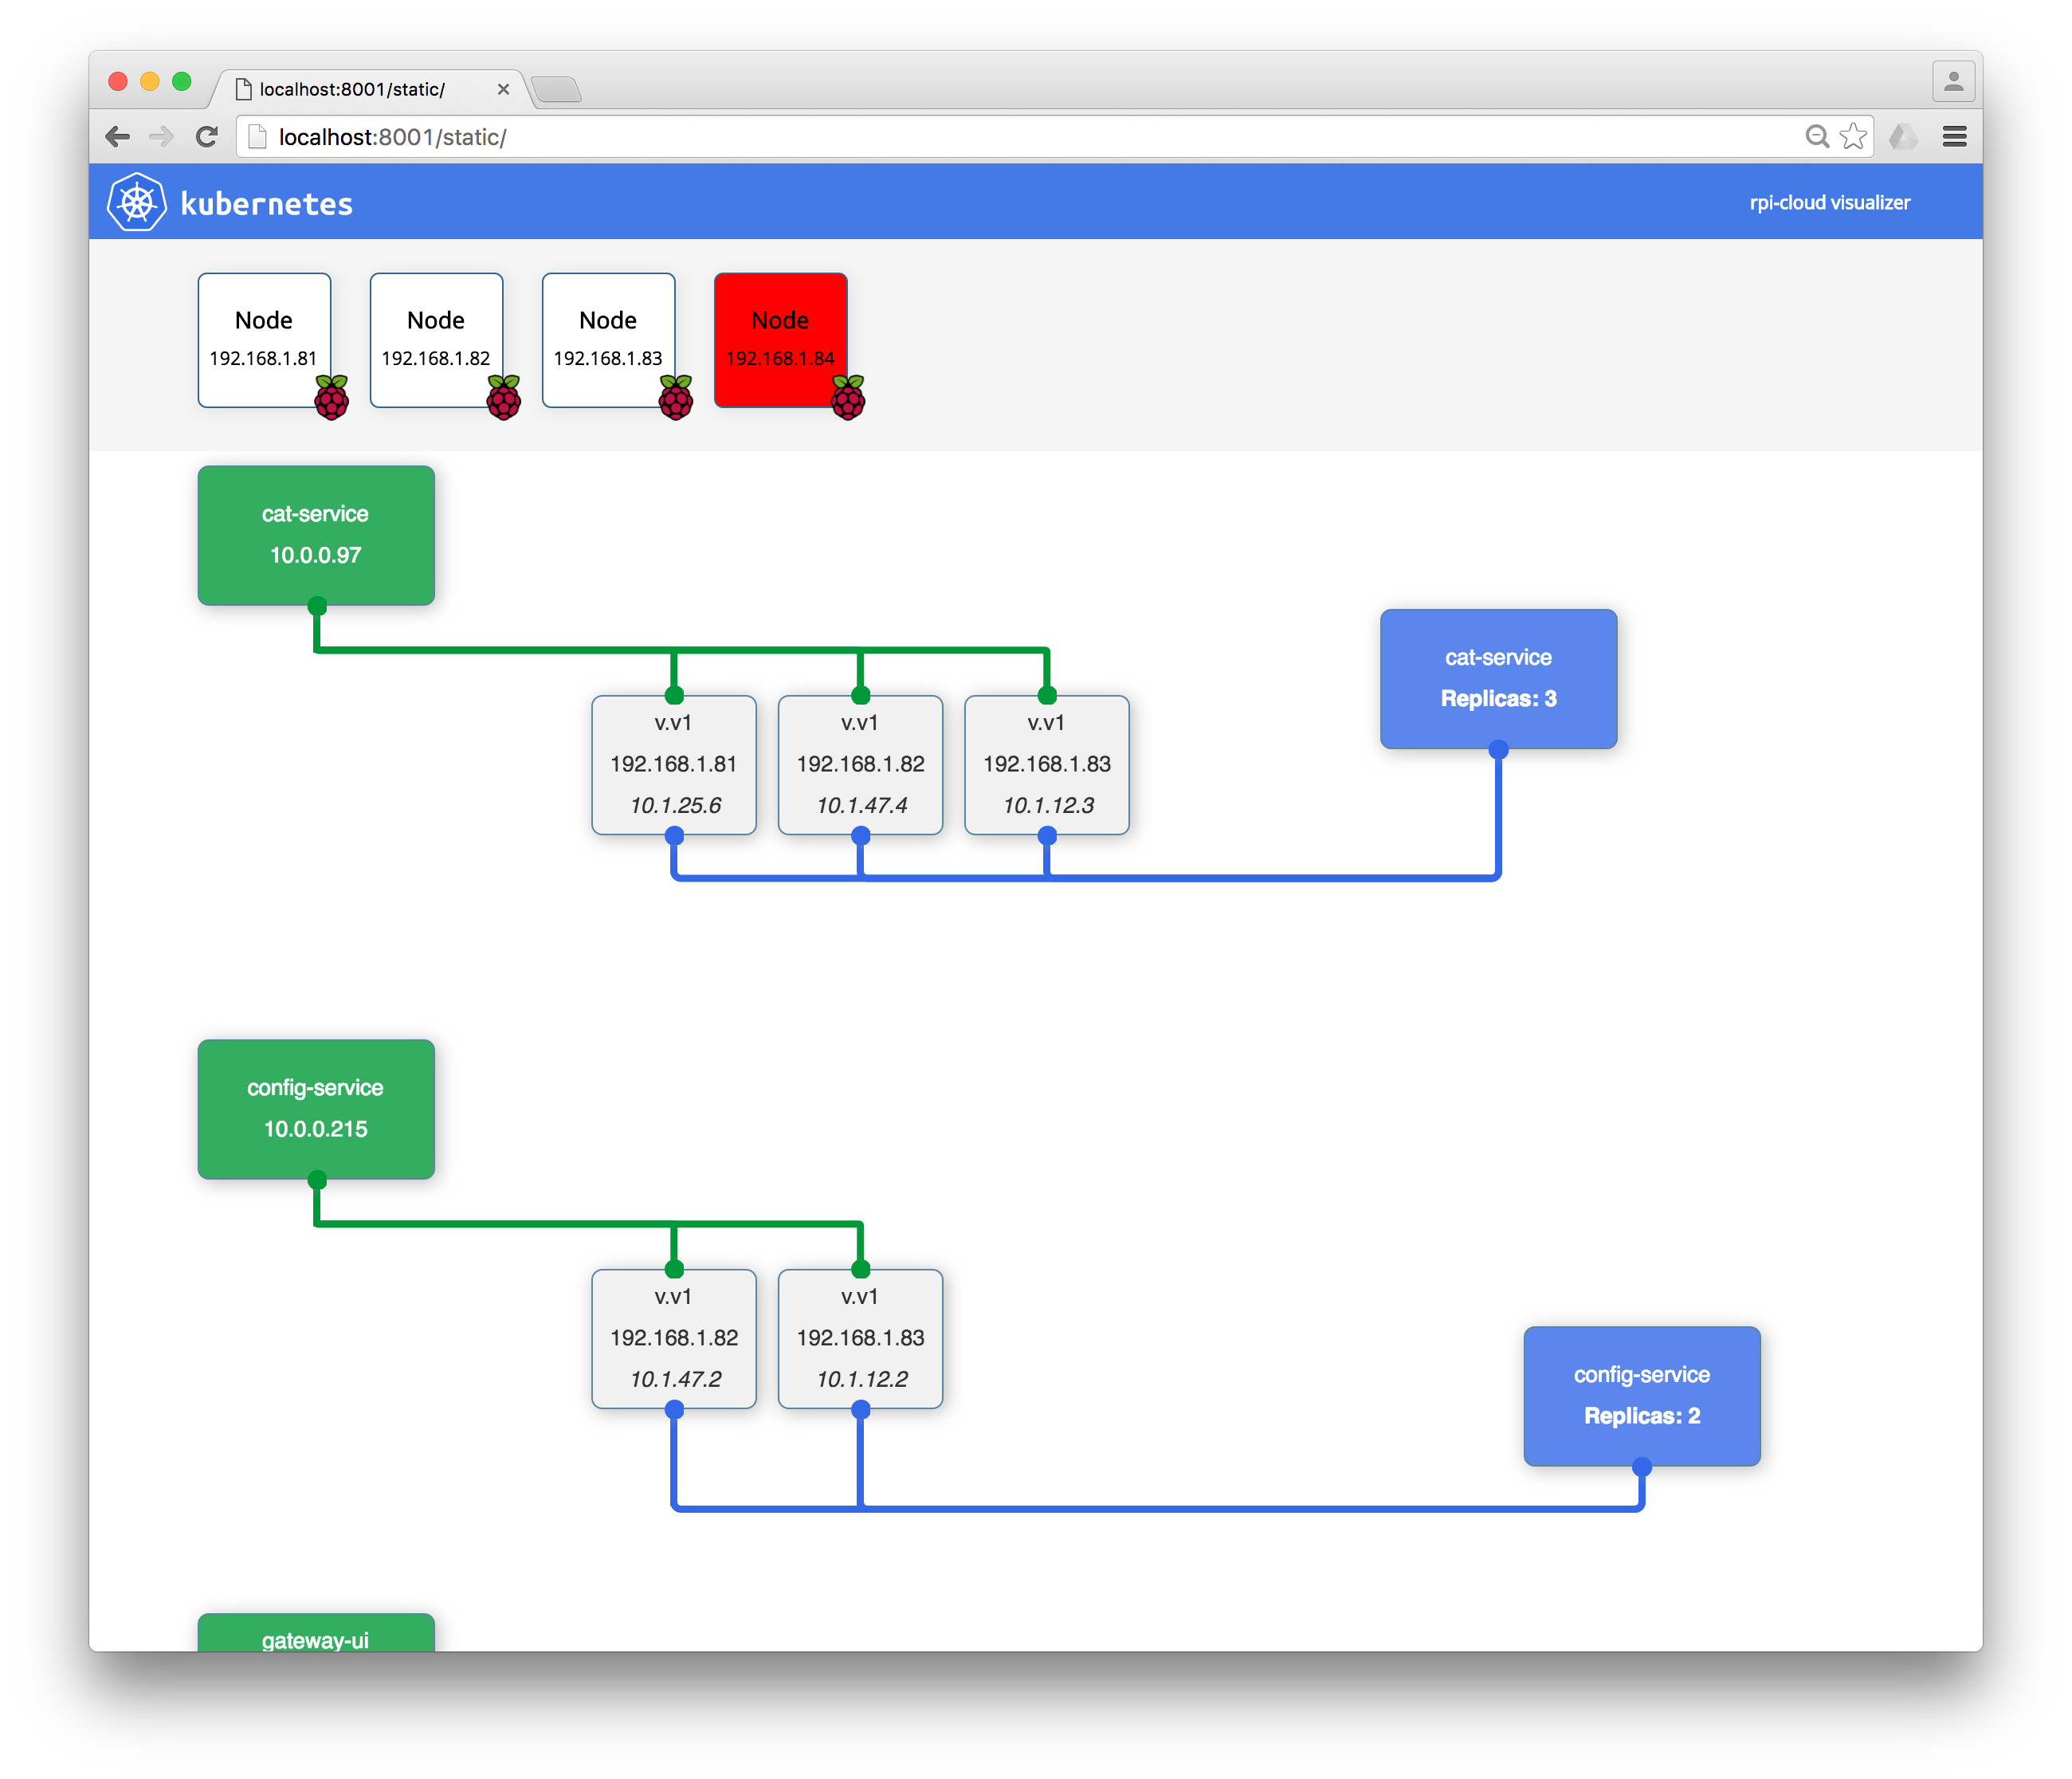
\includegraphics[width=7cm]{figures/visualizer/node_fail_recovered} }}%
    \caption{Visualization of Node Failure}%
    \label{fig:visualizer_node_failure}%
\end{figure}

\noindent 
The top row indicates the status of each node, and the red color indicates that the last node is not responding. Each green box corresponds to a running \textit{service}. The services are connected to \textit{pods} of varying colors. The pod color indicates whether a pod is running, pending or terminating. The pods are controlled by \textit{deployments} that are shown as blue boxes. \\
As seen in Figure~\ref{fig:visualizer_node_failure}, the overview of the cluster changes dynamically when the state of the cluster is changed. Figure~\ref{fig:visualizer_node_failure}(a) shows that one of the nodes is not reporting heartbeats to the API server. (b) shows Kubernetes rescheduling the pod running on the failing node to maintain the desired state of the deployment. (c) shows the recovery to the desired state. Lastly (d) everything is cleaned up and fully recovered.

\noindent
Brendan Burns, co-founder of the Kubernetes project, has created the original visualization tool. This tool has been open sourced and a lot of contributions have been made by, among others, Ray Tsang (saturnism) and Arjen Wassink (awassink). We have forked their repository and made some additions. The additions to the visualizer made during this master's thesis are, among others, fixing a memory leak in the original code. Drawing of nodes in the DOM kept being overlayed every 3 seconds. The result of having the visualizer open for longer periods made it heavy to interact with. Furthermore, the upgrade from Kubernetes 1.1 to 1.2 resulted in issues. ReplicationController were substituted with replica sets and deployments. We updated the visualizer to work with 1.2.